\documentclass[border=6pt]{standalone}
\usepackage{tikz}\usetikzlibrary{positioning,arrows.meta,fit,backgrounds,calc}
\usepackage[T1]{fontenc}\usepackage{lmodern}
\definecolor{slate}{RGB}{48,56,68}\definecolor{accent}{RGB}{198,102,36}\definecolor{mute}{RGB}{120,128,138}
\begin{document}
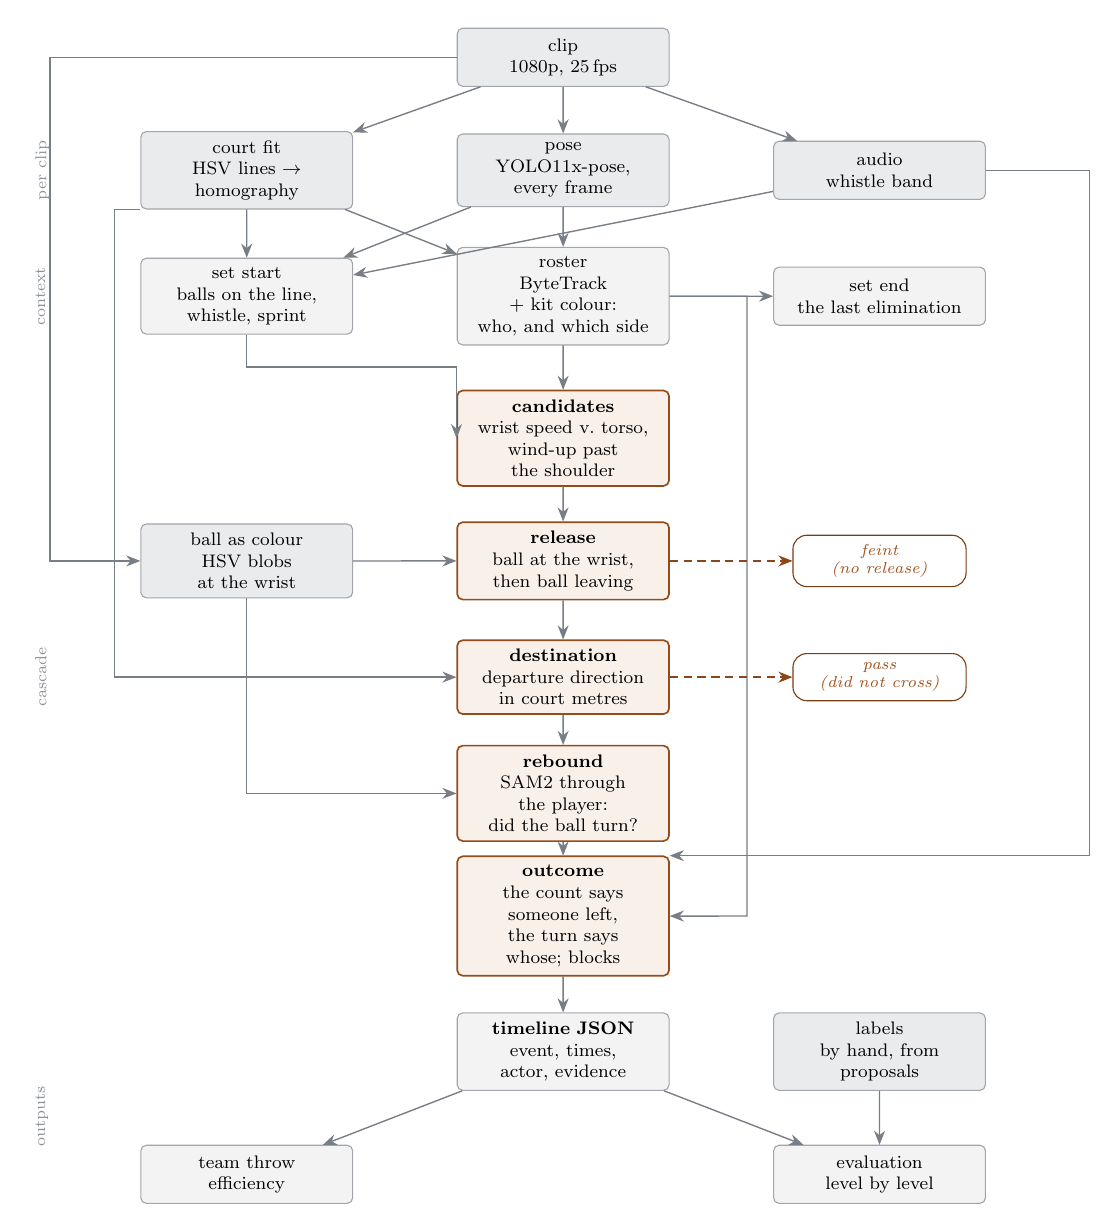
\begin{tikzpicture}[
  scale=0.82, every node/.style={transform shape},
  font=\small,
  stage/.style={draw=slate!55, fill=white, rounded corners=2pt, align=center,
                inner sep=4pt, minimum height=9mm, text width=30mm, font=\footnotesize},
  src/.style={stage, fill=slate!10, draw=slate!45},
  cas/.style={stage, draw=accent!75!black, fill=accent!10, line width=0.6pt},
  res/.style={stage, fill=slate!6, draw=slate!45},
  term/.style={draw=accent!60!black, fill=white, rounded corners=5pt, align=center,
               inner sep=4pt, text width=24mm, font=\scriptsize\itshape,
               text=accent!80!black},
  ar/.style={-{Stealth[length=1.8mm,width=1.4mm]}, draw=slate!65, line width=0.5pt},
  dar/.style={ar, densely dashed, draw=accent!70!black},
  lay/.style={font=\scriptsize, text=slate!55, anchor=west},
]

\node[src] (vid) at (0,0) {clip\\1080p, 25\,fps};

\node[src] (court) at (-4.9,-1.75) {court fit\\HSV lines $\to$ homography};
\node[src] (pose)  at (0,-1.75)    {pose\\YOLO11x-pose,\\every frame};
\node[src] (audio) at (4.9,-1.75)  {audio\\whistle band};

\node[res] (ss)    at (-4.9,-3.7) {set start\\balls on the line, whistle, sprint};
\node[res] (ros)   at (0,-3.7)    {roster\\ByteTrack $+$ kit colour:\\who, and which side};
\node[res] (se)    at (4.9,-3.7)  {set end\\the last elimination};

\node[cas] (cand) at (0,-5.9) {\textbf{candidates}\\wrist speed v.\ torso,\\wind-up past the shoulder};
\node[cas] (rel)  at (0,-7.8) {\textbf{release}\\ball at the wrist,\\then ball leaving};
\node[cas] (dest) at (0,-9.6) {\textbf{destination}\\departure direction\\in court metres};
\node[cas] (reb)  at (0,-11.4) {\textbf{rebound}\\SAM2 through the player:\\did the ball turn?};
\node[cas] (outc) at (0,-13.3) {\textbf{outcome}\\the count says someone left,\\the turn says whose; blocks};

\node[src] (ball) at (-4.9,-7.8) {ball as colour\\HSV blobs at the wrist};

\node[res] (tl)   at (0,-15.4) {\textbf{timeline JSON}\\event, times,\\actor, evidence};
\node[res] (met)  at (-4.9,-17.3) {team throw\\efficiency};
\node[res] (ev)   at (4.9,-17.3) {evaluation\\level by level};
\node[src] (lab)  at (4.9,-15.4) {labels\\by hand, from proposals};

\node[term] (fake) at (4.9,-7.8) {feint\\(no release)};
\node[term] (pass) at (4.9,-9.6) {pass\\(did not cross)};

\draw[ar] (vid) -- (court);
\draw[ar] (vid) -- (pose);
\draw[ar] (vid) -- (audio);
\draw[ar] (vid.west) -- ++(-6.3,0) |- (ball.west);

\draw[ar] (pose)  -- (ss);
\draw[ar] (audio) -- (ss);
\draw[ar] (court) -- (ss);
\draw[ar] (pose)  -- (ros);
\draw[ar] (court) -- (ros);
\draw[ar] (ros)   -- (se);

\draw[ar] (ros) -- (cand);
\draw[ar] (ss.south) -- ++(0,-0.5) -| (cand.west);
\draw[ar] (cand) -- (rel);
\draw[ar] (ball) -- (rel);
\draw[ar] (rel)  -- (dest);
\draw[ar] (dest) -- (reb);
\draw[ar] (reb) -- (outc);
\draw[ar] (ball.south) |- (reb.west);
\draw[ar] (court.south west) -- ++(-0.4,0) |- (dest.west);
\draw[ar] (ros.east) -- ++(1.2,0) -- ++(0,-9.6) -- (outc.east);
\draw[ar] (audio.east) -- ++(1.6,0) |- (outc.north east);

\draw[dar] (rel.east)  -- (fake.west);
\draw[dar] (dest.east) -- (pass.west);

\draw[ar] (outc) -- (tl);
\draw[ar] (tl)  -- (met);
\draw[ar] (tl)  -- (ev);
\draw[ar] (lab) -- (ev);

\node[lay] at (-8.3,-1.75) {\rotatebox{90}{\makebox[0pt]{per clip}}};
\node[lay] at (-8.3,-3.7)  {\rotatebox{90}{\makebox[0pt]{context}}};
\node[lay] at (-8.3,-9.6)  {\rotatebox{90}{\makebox[0pt]{cascade}}};
\node[lay] at (-8.3,-16.4) {\rotatebox{90}{\makebox[0pt]{outputs}}};

\end{tikzpicture}
\end{document}
